\lettrine{I}{n this chapter I present} the results of the models that have been specified in the previous chapter. What I find is that there is no evidence that linkages to China is influencing the level of freedom of expression in a country. This result does not change even when considering different types of regimes, which I theorised might behave differently when developing stronger links to China. This result is stable across different specifications. The one exemption is that I found a strong negative effect on hybrid regimes with a ten year lead on the dependent variable. This is not directly implausible, but I consider the time span and variation in the data to too great, making this a spurious relationship. 

I start this chapter by giving a few examples of how linkages to China and freedom of expression has co-varied over the time span in consideration (1994-2023).  This is a descriptive exercise to see if the theory is plausible. After this I turn to the results of the model estimations. I present and explaining how the results might be interpreted, noting some of the more interesting details. This chapter ends with a discussion on the validity, reliability, and the robustness of the results, as there are many ways in which to model data, and even small changes may have large impacts on the results.

\section{Examples}
\begin{table}[!hbt]
\centering
\caption{Changes in freedom of expression and linkages to China}
\label{tab:change}
\vspace{0.5em}
\begin{tabular}{lLp{15mm}lL}
\toprule
Country & \multicolumn{1}{c}{Freedom} & & Country & \multicolumn{1}{c}{Linkage} \\
\midrule
\cellcolor[HTML]{ff9214} Timor-Leste & 0.776 & & 
\cellcolor[HTML]{ff9214} Cambodia & 0.394 \\
Maldives & 0.636 & & Laos & 0.326 \\
Tunisia & 0.533 & & Turkmenistan & 0.314 \\
Libya & 0.531 & & Malaysia & 0.302 \\
Iraq & 0.510 & & Angola & 0.924 \\
\addlinespace
Hong Kong & -0.568 & & Tunisia & 0.018 \\
Venezuela & -0.670 & & Romania & -0.031 \\
Belarus & -0.735 & & Iran & -0.034 \\
Russia & -0.735 & & The Gambia & -0.067 \\
\cellcolor[HTML]{003F5C}\textcolor{white}{Nicaragua} & -0.869 &  &
\cellcolor[HTML]{003F5C}\textcolor{white}{North Korea} & -0.201 \\
\bottomrule
\multicolumn{5}{p{0.7\textwidth}}{\raggedright{\textit{For freedom score the the difference is measured between 1994 and 2024 \citep{coppedge_v-dem_2025}, while for linkage score it is the difference between 1994 and 2023 \citep{moyer_china-us_2021}.}}}
\end{tabular}
\end{table}

I want to start this section by examining some countries in greater detail to look at how our dependent and independent variables have changed over the time frame we are looking at. For freedom of expression I have data from 1994 to 2024 and for linkages to China I have data from 1994 to 2023. 

Are there any signs that the main hypothesis is true? I have chosen four countries, based on their scores on the two main variables. These are: Timor-Leste, with the largest increase in freedom of expression score; Nicaragua, with the largest decrease in freedom of expression score; Cambodia, with the largest increase in linkages with China; and North Korea, with the largest decrease in linkages with China. The top and bottom five of both dependent and independent variables can be seen in Table \ref{tab:change}.

\begin{figure}[!hbt]
    \centering
    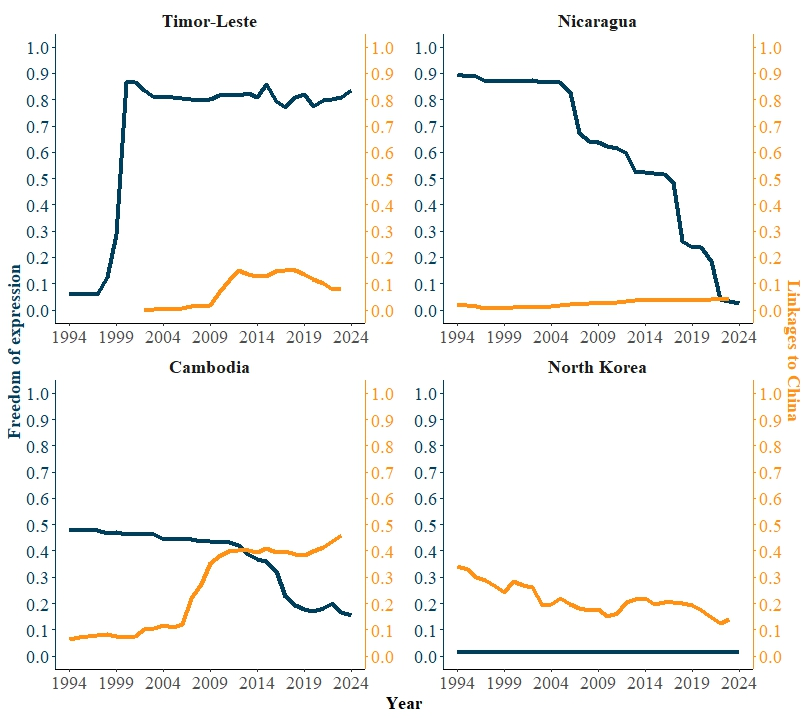
\includegraphics[width=\linewidth]{graphics/single_country_plots.jpeg}
    \caption{Change in linkages to China and freedom of expression (1994-2023/4)}
    \label{fig:scp}
\end{figure}


\subsection{Timor-Leste}
Timor-Leste, also known as East Timor, is a small country in Southeast Asia, located on the east part of the island of Timor, which it shares with its larger neighbour Indonesia. The country has had a fraught history, that reached its climax in 1999, when the country became independent from Indonesia after 24 years of occupation \citep[p. 183]{kingsbury_democratic_2014}. In Figure \ref{fig:scp} we can see that there is a large jump in the freedom of expression score in 1999, going from a score as low as 0.06 in 1997 to reaching a high of 0.87 in 2000. After which the score has decreased somewhat, but has held stable. While the FBIC index do not include scores for Timor-Leste before 2002, linkages to China only began rising around 2010, but this has not seemed to impact freedom of expression to any significant degree.

In the case of Timor-Leste it is independence from Indonesia which facilitated the rapid increase in freedom of expression. This is to highlight that, while linkages to China might have an effect, they can easily be drowned out by the noise of domestic realities, or at least problems much closer to home.

\subsection{Nicaragua}
Nicaragua is a poor Central American country, with a turbulent modern history, which shows in the decline of freedom of expression in the country. Since 2006, freedom of expression has declined rapidly under the leadership of Daniel Ortega, who, colluding with the opposition president, from 2000 gradually managed to gain more and more power, essentially being able to effect executive aggrandisement from a minority position \citep{mcconnell_elite_2024}.

While linkages to China have slowly increased between 1994 and 2023, this has happened at a very slow pace, and in absolute numbers they are very low. The reason for this is that Nicaragua has long recognised Taiwan as being the official China, to which China is not amicably disposed. This state of affairs, however, ended in 2021 when the country broke of diplomatic contact with the island nation \citep{bbc_nicaragua_2021}. Nicaragua's recognition of Taiwan has long limited relations with China, but I expect that the change of recognition will cause linkages between China and Nicaragua to expand dramatically in the future. However, as this is a recent development, this has not had the time to appear in the data. 

China most likely does not have much impact on Nicaragua, but this might not mean that linkages are not in play, just not linkages to China. \citet[p. 198]{mcconnell_elite_2024} argues that Black Knight authoritarian allies have had a great deal of influence, with Venezuela taking the lead. At the same time she emphasises domestic elite explanations, where the Black Knights are ancillary to domestic processes.

\subsection{Cambodia}
Cambodia is a country on the Indochinese peninsula, which was not spared the ravages of the Cold War, hosting one of the most brutal regimes the world has ever seen in the communist Khmer Rouge. It did subsequently democratise; however, this was never very successful, quickly becoming more authoritarian. In this autocratisation process freedom of expression has taken a large hit. At first this process was slow, with the country recording a slow but persistent decline in freedom of expression in the period between 1994 and 2012. This changed in 2012 as the score declined rapidly, before re-stabilising at a low level.

It is telling that the repression on freedom of expression began in earnest after a rapid increase in ties to China. The two lines in Figure \ref{fig:scp} seem almost to mirror each other, giving, at least a superficial impression, that there is a connection. This is substantiated by \citet{loughlin_chinese_2021}, who finds that the ruling Cambodian People's Party (CPP) has been both learning from and supported itself on China

\subsection{North Korea}
The last country I want to look at is North Korea, commonly labelled the hermit kingdom for its super-authoritarian and repressive regime. Its system is founded on self-reliance or Juche, with a strong cult of personality surrounding the ruling Kim clan. North Korea occupies the northern half of the Korean peninsula, and is almost entirely reliant on support from China as it faces crushing sanctions from the West. However, after the Russian invasion of Ukraine in 2022 Russia has become a much closer partner.

We see from the blue line in Figure \ref{fig:scp} that freedom of expression in North Korea is non-existent. North Korea is probably the most repressive regime on earth and there is no freedom to be had for a citizen. This has not changed even slightly in the last thirty years. The yellow line shows North Korea's linkages to China. This has fallen in recent years, which might either be because North Korea is diversifying its foreign policy or that China has become less eager to engage with the country, especially from 2006 when Pyongyang conducted its first nuclear weapons test \citep{fong_understanding_2024}. Whatever the case, the weakening of linkages to China in this period seems to have had no effect on freedom of expression in North Korea.

\section{Statistical Significance}
Before proceeding with the analysis, I will make a quick rejoinder on statistical significance. The reason is that I will refer to statistical significance as a convention. However, significance is an arbitrarily chosen threshold; being the point where we consider a result to be plausible enough that we reject the null-hypothesis and accept the results as being `true.' The most accepted threshold goes at the five per cent level (\citeauthor{christophersen_introduksjon_2018} \citeyear{christophersen_introduksjon_2018}, pp. 27-31; \citeauthor{gelman_regression_2021} \citeauthor{gelman_regression_2021}, p. 57; \citeauthor{halperin_political_2020} \citeyear{halperin_political_2020},  p. 432; \citeauthor{hellevik_forskningsmetode_2002} \citeyear{hellevik_forskningsmetode_2002}, p. 375; \citeauthor{kellstedt_fundamentals_2018} \citeyear{kellstedt_fundamentals_2018}, pp. 165-166), meaning that if we do the study 100 times, we can expect that in 95 of them of them we end up with a coefficient that is different from zero, and we can plausibly reject the null-hypothesis.

There is a tendency in the statistical community to be over-reliant on significance testing \citep{barnett_examination_2019, gelman_regression_2021, imbens_statistical_2021, van_zwet_significance_2021}. This is a problem as it incentivise researchers to aim for statistical significance, to the detriment of gaining true insight. We should therefore not be too concerned about significance, but use it as a rough way to distinguish the probable from the improbable.

When considering significance we should be aware of two points: one is that the effect should be large enough to be of consequence and the other is that we have enough observations. I will be discussing effect size later, especially in Section \ref{sec:effect}. My models varies between 5,154 and 3,473 observations. This is a fair number of observations, but in some cases, especially when adding an interaction term of a four-levelled factor variable (Table \ref{tab:h2}), it might not be enough to get a significant result, even if there is an effect. This is important to have in mind when trying to make sense of the results.

\section{Hypothesis One} \label{sec:h1}
In this section and the next, I present the results of the first regression model from the research design chapter, where I gradually include controls to test the stability of the results (Table \ref{tab:h1}). As a quick reminder, hypothesis one states that: \textit{thicker linkages to China will have a negative effect on the level of freedom of expression.} In addition to Table \ref{tab:h1}, I also include a table showing the fully specified model with different amounts of lead on the dependent variable (Table \ref{tab:h1_lead}). I do this to ensure that the effect is not obscured by  linkages taking time to be have an effect. All models use two-way fixed-effects to control for country and time invariables, as this is likely to be a source of unobserved variable bias if they remain uncontrolled for. Because there is a high likelihood that there are considerable differences in the standard errors of the units, I cluster the standard errors by country, making them robust to unit heterogeneity. For readability, I have also decided to highlight the linkages to China variable in the regression tables. It will be orange if there are no significant finds, and blue if the coefficients are significant at the five per cent level. This should, however, only be thought of as a reading aid. 

\subsection{Relationship between linkages to China and freedom of expression}
\begin{table}[H]
\centering
\resizebox{\textwidth}{!}{
\begin{talltblr}[         %% tabularray outer open
label=tab:h1,caption={Standard two-way fixed-effects models},
note{}={x p \num{< 0.1}, * p \num{< 0.05}, ** p \num{< 0.01}, *** p \num{< 0.001}},
]                     %% tabularray outer close
{                     %% tabularray inner open
colspec={Q[]Q[]Q[]Q[]Q[]Q[]Q[]},
column{2,3,4,5,6,7}={}{halign=c,},
column{1}={}{halign=l,},
hline{18}={1,2,3,4,5,6,7}{solid, black, 0.05em},
}                     %% tabularray inner close
\toprule
& \textbf{Model 1.1} & \textbf{Model 1.2} & \textbf{Model 1.3} & \textbf{Model 1.4} & \textbf{Model 1.5} & \textbf{Model 1.6} \\ \midrule %% TinyTableHeader
\SetCell{bg=Orange} Linkages to China &
\SetCell{bg=Orange} -0.081 & 
\SetCell{bg=Orange} -0.093 & 
\SetCell{bg=Orange} -0.069 & 
\SetCell{bg=Orange} -0.067 & 
\SetCell{bg=Orange} -0.111 & 
\SetCell{bg=Orange} -0.058 \\
& (0.132) & (0.134) & (0.127) & (0.128) & (0.130) & (0.111) \\
log(GDP per capita) &  & 0.009 & 0.001 & 0.008 & 0.016 & -0.003 \\
&  & (0.019) & (0.020) & (0.022) & (0.023) & (0.020) \\
Resource rents &  &  & 0.000 & 0.000 & 0.000 & 0.000 \\
&  &  & (0.001) & (0.001) & (0.001) & (0.001) \\
Aid &  &  &  & 0.001 & 0.001 & 0.002** \\
&  &  &  & (0.001) & (0.001) & (0.001) \\
Linkages (West) &  &  &  &  & -0.023* & -0.016x \\
&  &  &  &  & (0.012) & (0.009) \\
Electoral autocracy &  &  &  &  &  & 0.085** \\
&  &  &  &  &  & (0.030) \\
Electoral democracy &  &  &  &  &  & 0.238*** \\
&  &  &  &  &  & (0.034) \\
Liberal democracy &  &  &  &  &  & 0.285*** \\
&  &  &  &  &  & (0.037) \\
Num.Obs. & 5154 & 5150 & 4657 & 4648 & 4648 & 4648 \\
Std.Errors & by: country & by: country & by: country & by: country & by: country & by: country \\
R2 Adj. & 0.874 & 0.874 & 0.882 & 0.883 & 0.883 & 0.907 \\
R2 Within Adj. & 0.001 & 0.001 & 0.000 & 0.003 & 0.008 & 0.208 \\
FE: country & X & X & X & X & X & X \\
FE: year & X & X & X & X & X & X \\
\bottomrule
\end{talltblr}
}
\end{table} 

Table \ref{tab:h1} includes six different versions of Model 1, estimating the effect of linkages to China on freedom of expression. Model 1.6, the most complex, is equivalent to Equation \ref{equ:h1} above. Model 1.1 regress linkages to China directly on freedom of expression without including any control variables. I then gradually include the five control variables described in Section \ref{control}. The first control variable I include is the logged GDP per capita variable (Model 1.2), the second is total natural resources rents as a percentage of GDP (Model 1.3), the third is Official Development Assistance, better known as aid, which is measured as per cent of GNI (Model 1.4), the fifth is linkages to the West, an aggregate of linkages to Western countries (Model 1.5), and the final model introduces the regime control variable, a factor variable of four levels, with closed autocracies being the reference value (Model 1.6), giving us the full model.  I start with 5,154 observations, and in the last model I end up with 4,648, losing 506 observation through missingness on the control variables. The biggest loss of observations happens when including the total natural resources rents variable in model 1.3, because this variable only has data up until 2021. All the models are all using country and time fixed effects, with the freedom of expression scores being lead by one year to exclude reversed causation. 

The highlighted row labelled Linkages to China shows us the main effect we are after, namely the effect of linkages to China on freedom of expression. The sign of this coefficient is negative in all cases, indicating that linkages to China have a negative effect on freedom of expression. However we see that the effect sizes are small and the standard errors are large so we cannot be confident in this relationship. Other than this, there are a few more things to note. First, the coefficient for GDP per capita is non-significant and small, probably indicating that most of the variation in this variable is controlled for by using fixed effects. Second, that aid is significant only when also controlling for regime type. Third, that linkages to the West is negative and statistically significant in Model 1.5, but the significance disappears when controlling for regime type. This is very surprising in light of earlier studies \citep{levitsky_linkage_2006}, however, I will explore this further below in the discussion chapter. And fourth, that regime type is always positive and statistically significant. This latter observation is unsurprising as one, all the regime types are more democratic than the reference regime type which is closed autocracy, and two, because the regime variable is partially based on the freedom of expression variable.

It can be clearly seen in Table \ref{tab:h1} that linkages to China does not have a direct impact on freedom of expression scores. While the sign of the linkage variable is indeed negative, the standard error is quite large, being more than twice the size of the estimated effect in all models.

\subsection{Different time leads}
I also test how the model reacts when using different time leads. I do this by using the most complex model from Table \ref{tab:h1} (Model 1.6). I test for five additional time leads in Table \ref{tab:h1_lead}, starting with a lead if two years in Model 1.7, four in Model 1.8, six in Model 1.9, eight in Model 1.10, and finally ten in Model 1.11. From the example of Cambodia in Figure \ref{fig:scp}, it seems like linkages take time before they have effect, and this should be investigated further.

The size of the coefficient for linkages to China increases up until an eight year lag, before it decreases again. The sign is negative and the effect becomes somewhat sizeable. However the standard error is still large and never reaches the five per cent threshold of statistical significance, meaning that we should consider it implausible that linkages to China have an effect on freedom of expression. 

What is more interesting to see is that linkages to the West is negative and statistically significant for all leads. It means that if a country increases its linkages to the West, the model predicts that freedom of expression decreases. We should also note that the regime factor variables all lose significance and coefficient size. This is expected as the further removed from the freedom of expression score in time, the less they should be able to predict it. 

\begin{table}[H]
\centering
\resizebox{\textwidth}{!}{
\begin{talltblr}[         %% tabularray outer open
label=tab:h1_lead,caption={Model 1.6 with different leads},
note{}={x p \num{< 0.1}, * p \num{< 0.05}, ** p \num{< 0.01}, *** p \num{< 0.001}},
]                     %% tabularray outer close
{                     %% tabularray inner open
colspec={Q[]Q[]Q[]Q[]Q[]Q[]},
column{2,3,4,5,6}={}{halign=c,},
column{1}={}{halign=l,},
hline{18}={1,2,3,4,5,6}{solid, black, 0.05em},
}                     %% tabularray inner close
\toprule
& \textbf{Model 1.7} & \textbf{Model 1.8} & \textbf{Model 1.9} & \textbf{Model 1.10} & \textbf{Model 1.11} \\ \midrule %% TinyTableHeader
\SetCell{bg=Orange} Linkages to China &
\SetCell{bg=Orange} -0.088 & 
\SetCell{bg=Orange} -0.188 & 
\SetCell{bg=Orange} -0.278x & 
\SetCell{bg=Orange} -0.318x & 
\SetCell{bg=Orange} -0.272 \\
& (0.118) & (0.137) & (0.156) & (0.175) & (0.184) \\
log(GDP per capita) & 0.003 & 0.013 & 0.017 & 0.012 & 0.001 \\
& (0.020) & (0.022) & (0.021) & (0.017) & (0.016) \\
Resource rents & 0.000 & 0.000 & 0.000 & 0.000 & 0.000 \\
& (0.001) & (0.001) & (0.001) & (0.001) & (0.001) \\
Aid & 0.002* & 0.001 & 0.001 & 0.000 & 0.000 \\
& (0.001) & (0.001) & (0.001) & (0.001) & (0.001) \\
Linkages (West) & -0.020* & -0.027* & -0.031* & -0.034* & -0.035* \\
& (0.009) & (0.011) & (0.012) & (0.013) & (0.014) \\
Electoral autocracy & 0.063* & 0.028 & 0.008 & 0.002 & -0.015 \\
& (0.028) & (0.026) & (0.025) & (0.024) & (0.026) \\
Electoral democracy & 0.192*** & 0.112*** & 0.061* & 0.037 & 0.017 \\
& (0.032) & (0.029) & (0.027) & (0.026) & (0.029) \\
Liberal democracy & 0.241*** & 0.165*** & 0.112** & 0.081* & 0.059x \\
& (0.035) & (0.034) & (0.035) & (0.034) & (0.034) \\
Num.Obs. & 4648 & 4484 & 4149 & 3812 & 3473 \\
Std.Errors & by: country & by: country & by: country & by: country & by: country \\
R2 Adj. & 0.899 & 0.894 & 0.897 & 0.899 & 0.903 \\
R2 Within Adj. & 0.149 & 0.073 & 0.042 & 0.030 & 0.026 \\
FE: country & X & X & X & X & X \\
FE: year & X & X & X & X & X \\
Lead freedom & 2 & 4 & 6 & 8 & 10 \\
\bottomrule
\end{talltblr}
}
\end{table} 

\section{Hypothesis two} \label{sec:h2}
In hypothesis two, I set out to study if the effect of linkages to China is regime dependent. It will be remembered from the last chapter of the theory section that hypothesis two states: \textit{Thicker linkages to China will have a greater negative effect on the level of freedom of expression in hybrid regimes}. To assess the veracity of this hypothesis, I add an interaction term between the linkages to China variable and the regime variable. The resulting interactions show the effect of linkages on a certain type of regime, with closed autocracies being the reference category. For the purposes of hypothesis two, I consider closed autocracies and liberal democracies to be `consolidated regimes,' while electoral autocracies and democracies are consider hybrid regimes. All the other specifications are similar to hypothesis one. 

\subsection{Relationship between linkages to China and freedom of expression by regime type}

\begin{table}[!hbt]
\centering
\resizebox{\textwidth}{!}{
\begin{talltblr}[         %% tabularray outer open
label=tab:h2,caption={Relationship between linkages to China and freedom of expression including regime type interaction},
note{}={x p \num{< 0.1}, * p \num{< 0.05}, ** p \num{< 0.01}, *** p \num{< 0.001}},
]                     %% tabularray outer close
{                     %% tabularray inner open
colspec={Q[]Q[]Q[]Q[]Q[]Q[]},
column{2,3,4,5,6}={}{halign=c,},
column{1}={}{halign=l,},
hline{24}={1,2,3,4,5,6}{solid, black, 0.05em},
}                     %% tabularray inner close
\toprule
& \textbf{Model 2.1} & \textbf{Model 2.2} & \textbf{Model 2.3} & \textbf{Model 2.4} & \textbf{Model 2.5} \\ \midrule %% TinyTableHeader
\SetCell{bg=Orange} Linkages to China & 
\SetCell{bg=Orange} -0.047 & 
\SetCell{bg=Orange} -0.025 & 
\SetCell{bg=Orange} -0.096 & 
\SetCell{bg=Orange} -0.096 & 
\SetCell{bg=Orange} -0.124 \\
& (0.218) & (0.230) & (0.256) & (0.249) & (0.252) \\
\SetCell{bg=Orange} China x El.Aut. & 
\SetCell{bg=Orange} -0.044 & 
\SetCell{bg=Orange} -0.045 & 
\SetCell{bg=Orange} 0.113 & 
\SetCell{bg=Orange} 0.117 & 
\SetCell{bg=Orange} 0.115 \\
& (0.290) & (0.294) & (0.312) & (0.301) & (0.299) \\
\SetCell{bg=Orange} China x El.Dem. & 
\SetCell{bg=Orange} -0.090 & 
\SetCell{bg=Orange} -0.092 & 
\SetCell{bg=Orange} -0.018 & 
\SetCell{bg=Orange} -0.012 & 
\SetCell{bg=Orange} -0.004 \\
& (0.253) & (0.256) & (0.274) & (0.266) & (0.266) \\
\SetCell{bg=Orange} China x Lib.Dem. & 
\SetCell{bg=Orange} -0.238 & 
\SetCell{bg=Orange} -0.268 & 
\SetCell{bg=Orange} -0.207 & 
\SetCell{bg=Orange} -0.207 & 
\SetCell{bg=Orange} -0.126 \\
& (0.260) & (0.277) & (0.291) & (0.280) & (0.280) \\
log(GDP per capita) &  & -0.013 & -0.019 & -0.011 & -0.005 \\
&  & (0.017) & (0.018) & (0.019) & (0.020) \\
Resource rents &  &  & 0.000 & 0.000 & 0.000 \\
&  &  & (0.001) & (0.001) & (0.001) \\
Aid &  &  &  & 0.002** & 0.002** \\
&  &  &  & (0.001) & (0.001) \\
Linkages (West) &  &  &  &  & -0.014 \\
&  &  &  &  & (0.009) \\
Electoral autocracy & 0.094** & 0.097** & 0.071* & 0.075* & 0.074* \\
& (0.036) & (0.036) & (0.034) & (0.034) & (0.034) \\
Electoral democracy & 0.261*** & 0.265*** & 0.234*** & 0.237*** & 0.235*** \\
& (0.039) & (0.040) & (0.039) & (0.039) & (0.039) \\
Liberal democracy & 0.313*** & 0.318*** & 0.292*** & 0.295*** & 0.288*** \\
& (0.041) & (0.042) & (0.043) & (0.043) & (0.041) \\
Num.Obs. & 5154 & 5150 & 4657 & 4648 & 4648 \\
Std.Errors & by: country & by: country & by: country & by: country & by: country \\
R2 Adj. & 0.902 & 0.901 & 0.905 & 0.907 & 0.907 \\
R2 Within Adj. & 0.216 & 0.217 & 0.201 & 0.207 & 0.209 \\
FE: country & X & X & X & X & X \\
FE: year & X & X & X & X & X \\
\bottomrule
\end{talltblr}
}
\end{table} 

Table \ref{tab:h2} is almost the same as table Table \ref{tab:h1}, but this time linkages to China variable is interacted with the regime type variable. This has the unfortunate effect of complicating the model. However, making this adjustment, it is now possible to see the effect that linkages have on each regime type. To simplify the reading of the table, I am going to focus most of my attention on the highlighted rows, as these are the coefficients that are of main interest. The uppermost row of the table, labelled \textit{Linkages to China}, shows the results for closed autocracies, which is the reference category. In the next highlighted row we find the coefficients for the linkages to China for electoral autocracies, followed by the estimated coefficients for the effect of linkages to China for electoral democracies and liberal democracies respectively.

There are some interesting differences from the models being run in Section \ref{sec:h1}, but none of the coefficients showing the estimated effect of linkages to China are statistically significant. While it is consistently estimated that linkages to China have a negative effect on freedom of expression for more consolidated regimes, the coefficients for hybrid regimes are less stable, becoming positive for electoral autocracies in Model 2.3. Note particularly that the standard errors for all the models are large, being at best the same size as the effect itself, and sometimes much larger. The reason for this is that we divide the observations into four separate categories when estimating, dramatically lowering the ability of the model to estimate the relationship. The relationship also seems to be weak, making it hard to argue that China has any measurable effect on freedom of expression. 

The only significant result is that aid is estimated to be positively and significantly related to freedom of expression, however, the size of the coefficient is very small. Also, including the interaction term has removed the negative impact of linkages to the West, showing that this variable is possibly influenced by regime type. 

Considering this result with respect to the second hypothesis, there is no indication that hybrid regimes are more affected by linkages to China, than are consolidated regimes. In fact, based on this estimation, hybrid regimes looks to be, if anything, less effected by linkages to China. I believe this might come down to the fact that there is much greater variety for hybrid regimes in general, and that this model cannot capture this properly. This is to be discussed later. 


\subsection{Different time leads}
As for hypothesis one, I examine the results for the most complex model from Table \ref{tab:h2} for different time leads. I show this in Table \ref{tab:h2_lead}, where I use the same leads as for the previous table. There are some very interesting results in this table. Using a lead of two years, we see no significant results, and the effect sizes are small compared to the standard errors meaning we have a lot of uncertainty around them. When using a lead of four years, the effect decreases for all coefficients except the liberal democracy one. At six years the coefficient for closed autocracies reach its largest size and the coefficient for liberal democracy becoming positive. With an eight year lead, the effect size of closed autocracies shrinks, with all the other becoming more negative. With a ten year lead the results become very interesting. The coefficient of the closed autocracies becomes positive, the liberal democracy coefficient gets dramatically more negative. Then the estimated coefficients for the two electoral regime types become significant and strongly negative.

This result might at first seem to partially confirm hypothesis one and confirm hypothesis two. Hypothesis one is partially confirmed because linkages to China has an effect on freedom of expression, contingent on regime type. The second hypothesis is confirmed since the effect is much larger, and only significant, for hybrid regimes. I will, however caution against this interpretation. What this tells us is that an increase in linkages ten years previous is associated with a decrease in freedom of expression. While this is possible, it is very unlikely that a change would take ten years to manifest itself. Using a time span as long as this also removes a lot of information making it possible that we have created an artificial effect.

Another thing to note is that the coefficient for linkages to the West is consistently negative and significant. This is the same as in Table \ref{tab:h1_lead}.

\begin{table}[!htb]
\centering
\resizebox{\textwidth}{!}{
\begin{talltblr}[         %% tabularray outer open
label=tab:h2_lead,caption={Model 2.5 with different leads},
note{}={x p \num{< 0.1}, * p \num{< 0.05}, ** p \num{< 0.01}, *** p \num{< 0.001}},
]                     %% tabularray outer close
{                     %% tabularray inner open
colspec={Q[]Q[]Q[]Q[]Q[]Q[]},
column{2,3,4,5,6}={}{halign=c,},
column{1}={}{halign=l,},
hline{24}={1,2,3,4,5,6}{solid, black, 0.05em},
}                     %% tabularray inner close
\toprule
& \textbf{Model 2.6} & \textbf{Model 2.7} & \textbf{Model 2.8} & \textbf{Model 2.9} & \textbf{Model 2.10} \\ \midrule %% TinyTableHeader
\SetCell{bg=Orange} Linkages to China & 
\SetCell{bg=Orange} -0.127 & 
\SetCell{bg=Orange} -0.160 & 
\SetCell{bg=Orange} -0.176 & 
\SetCell{bg=Orange} -0.138 & 
\SetCell{bg=Orange}  0.123 \\
& (0.249) & (0.243) & (0.238) & (0.201) & (0.206) \\
\SetCell{bg=Orange} China x El.Aut. & 
\SetCell{bg=Orange}  0.085 & 
\SetCell{bg=Orange}  0.002 & 
\SetCell{bg=Orange} -0.103 & 
\SetCell{bg=Orange} -0.206 & 
\SetCell{bg=Blue} \textcolor{white}{-0.437*} \\
& (0.279) & (0.233) & (0.202) & (0.150) & (0.198) \\
\SetCell{bg=Orange} China x El.Dem. & 
\SetCell{bg=Orange} -0.069 & 
\SetCell{bg=Orange} -0.187 & 
\SetCell{bg=Orange} -0.250 & 
\SetCell{bg=Orange} -0.318 & 
\SetCell{bg=Blue} \textcolor{white}{-0.667*} \\
& (0.254) & (0.236) & (0.242) & (0.241) & (0.289) \\
\SetCell{bg=Orange} China x Lib.Dem. & 
\SetCell{bg=Orange} -0.092 & 
\SetCell{bg=Orange} -0.011 & 
\SetCell{bg=Orange}  0.018 & 
\SetCell{bg=Orange} -0.026 & 
\SetCell{bg=Orange} -0.229 \\
& (0.274) & (0.270) & (0.269) & (0.242) & (0.257) \\
log(GDP per capita) & 0.001 & 0.013 & 0.018 & 0.013 & 0.003 \\
& (0.020) & (0.022) & (0.021) & (0.018) & (0.017) \\
Resource rents & 0.000 & 0.000 & 0.001 & 0.000 & 0.000 \\
& (0.001) & (0.001) & (0.001) & (0.001) & (0.001) \\
Aid & 0.002* & 0.001 & 0.001 & 0.000 & 0.000 \\
& (0.001) & (0.001) & (0.001) & (0.001) & (0.001) \\
Linkages (West) & -0.019* & -0.027* & -0.032** & -0.036** & -0.037** \\
& (0.009) & (0.010) & (0.012) & (0.013) & (0.014) \\
Electoral autocracy & 0.054x & 0.026 & 0.016 & 0.016 & 0.011 \\
& (0.032) & (0.032) & (0.031) & (0.030) & (0.030) \\
Electoral democracy & 0.194*** & 0.123*** & 0.078* & 0.058x & 0.056 \\
& (0.037) & (0.036) & (0.035) & (0.034) & (0.035) \\
Liberal democracy & 0.245*** & 0.168*** & 0.116** & 0.088* & 0.081* \\
& (0.040) & (0.040) & (0.040) & (0.039) & (0.037) \\
Num.Obs. & 4648 & 4484 & 4149 & 3812 & 3473 \\
Std.Errors & by: country & by: country & by: country & by: country & by: country \\
R2 Adj. & 0.899 & 0.894 & 0.897 & 0.899 & 0.905 \\
R2 Within Adj. & 0.150 & 0.074 & 0.044 & 0.033 & 0.038 \\
FE: country & X & X & X & X & X \\
FE: year & X & X & X & X & X \\
Lead freedom & 2 & 4 & 6 & 8 & 10 \\
\bottomrule
\end{talltblr}
}
\end{table} 

\section{Understanding the coefficient} \label{sec:effect}
While the results are not significant, I want to illustrate the estimated effects. If they had been significant how strong would they be? First we need to know a bit more about the dependent and independent variables. Table \ref{tab:summary} includes some descriptive information of the variables. The freedom variable has a mean of 0.66 and a standard deviation of 0.29. For the linkage variable, we see that the mean is about 0.08, which is not a lot, considering the variable varies between 0 and 0.48. It also has a standard deviation of 0.08, which is not a lot.

\subsection{Linkages to China}
Using the estimates from Model 1.6 in Table \ref{tab:h1}, I will look at the what the coefficients tells us about two countries. If we had two perfectly similar countries: GDP per capita, resource rents, aid, linkages to the West, and regime type all being the same, a difference of 0.08 in the linkages to China variable---the standard deviation of said variable---is by Model 2.5 expected to lead to a:
\begin{equation*}
    (-0.058 \cdot 0.08) = -0.00464
\end{equation*}
lower freedom of expression score. Given that the standard deviation of the freedom variable is 0.29, this is close to nothing.

Now, lets also imagine that the country with more linkages to China continue to increase its ties with China by the same amount each year for a 15 year period. This would give us a predicted score of:
\begin{equation*}
    (-0.058 \cdot 0.08)\cdot 15 = -0.0696
\end{equation*}
Which is still very small. This is to say that, even had the coefficients been statistically significant, the effect would not have been substantial. This is unsurprising as for most countries, both the freedom score and linkage score is quite stable, with more dramatic changes occurring only sporadically, and are thus less likely to show evidence of a pattern.

\subsection{Linkages to the West} \label{sec:west_coefficients}
As it is interesting that the estimated coefficient for linkages to the West is significant across several specifications, I will also look at the size of this effect. I start as before with examining the summary statistics table \ref{tab:summary}. Linkages to the West have a standard deviation of 1.08. This is much more variation then for the linkage variable to China. Calculating the estimated effect for one year using model 1.6 gives us an estimated decrease in freedom of expression score of about 0.016, much smaller than the standard deviation in the variable. However, if we allow a country to grow its linkages to the West for 15 years, we get an estimated freedom of expression score that is:
\begin{equation*}
    (-0.016 \cdot 1.08)*15 = -0.2592
\end{equation*}
lower than for a similar country that has not increased its linkages to the West. This is a sizeable decrease in freedom of expression score, which seems quite peculiar. More on this in the discussion chapter below. 

\section{Robustness Tests} \label{sec:robust}
To test the robustness of the results, I run several different model specifications to see how well the models hold up to scrutiny. While I present the results here, all the tables referred to in this section can be found in Appendix \ref{apn:robust}. I make two major changes to my models, to assess how all the models in Tables \ref{tab:h1} and \ref{tab:h2} stand up to different forms of scrutiny. First I investigate how removing the one year time lead impacts the models. Then I replace the linkages to China variable, which heretofore have made use of the FBIC-variable, with the bandwidth variable also featured in the FBIC dataset \citep{moyer_china-us_2021}. Doing this ensures that the estimations are consistent in their results across different forms of specifications. I find that they are generally consistent, but with some differences.

\subsection{Models without lead on the dependent variable}
I next include four more tables running the four main tables of this chapter without lead. I do this to check if the effect might be immediate. I do not expect it to be, however, large discrepancies between models with and without lead should be investigated further. As a caveat to this, it is somewhat more likely that the models using change in linkages to China---instead of the absolute size of them---can be impacted by removing the lead, as they already account for some of the time difference. As I have already noted, the estimated coefficients of the models using change in linkages is larger the smaller the lead, and, in the case of change in the independent variable, the possibility of reversed causation is by definition excluded. This means that we should take very seriously any change in the estimates when using change in linkages as the main independent variable.

Tables \ref{tab:h1_x_lead} and \ref{tab:h2_x_lead} shows no significant changes from the models in the analysis chapter. The estimated coefficients are a little different, but nothing that would change any conclusions. Removing the lead only have smaller impacts on our estimations. While the results was not consistent with my speculation about how the models running variables with change would be affected, they are nonetheless conforming mostly to expectations.


\subsection{Bandwidth}
The last specification I run uses the `bandwidth' variable which is one of the two parts that make up the FBIC index main variable. I include models using this variable to see how removing the importance of the linkages affects the estimations. Bandwidth measures the number of linkages, but not how important these are to the partner of China. According to \citet{levitsky_linkage_2006}, linkages are the main way through which democracy can be spread, with leverage mainly working to strengthen the effects of the linkages. The number of linkages, then, is more important than their size according to this theory. On this basis I include models using bandwidth to check the stability of the results. Again, I rerun all the models in the four main tables of this chapter.

What I find when using bandwidth as the independent variable, is that the models from Table \ref{tab:h1} barely change at all (see Table \ref{tab:h1_bandwidth}). The same is true for Table \ref{tab:h2} (see Table \ref{tab:h2_bandwidth}).Using bandwidth affect the size of the estimates, however, the sign is the same. This is expected as bandwidth leaves out some of the information from the main FBIC variable. We can conclude that using the bandwidth variable does not affect the stability of the results in a way that would invalidate them. 

\section{Residuals}
We also need to take a look at residuals to check whether or not there are any problems. I have selected to only focus on the residual plot of Model 2.5, as all the models have residual plots very similar to one another.

A residual plot for a model with a good fit should be narrow, with random clustering around zero for every residual. The narrowness means that the model predicts values well for all observations and the clustering around zero means that the estimates are unbiased, commonly known as homoscedasticity. This is not the case with these models, and here I will explain why this is, what the problem is and how I have proceeded to rectify this.

The residual plot of Model 2.5 is shaped like a diamond around zero. This is to say that the residuals are heteroscedastic, i.e., that different observations have different prediction errors. While the model is fairly good at predicting observations that have either low or high freedom of expression scores, it struggles with values that are somewhere in the middle. The reason is quite simple, in that there is an upper and lower limit to the dependent variable, and when coming close to this limit the rate of change decreases dramatically, resulting in better estimates. We should also expect there to be some considerable outliers, because of domestic factors like coups or newly gained independence. Because of their nature, these are outliers which the model should not be able to predict. In Figure \ref{fig:residuals} I have highlighted some of the worst predicted observations, which in most cases are countries where large changes have occurred, for instance Afghanistan in 2020-2021 and the Gambia in 2016. 

The good thing about the model is that it is unbiased, thus the coefficients should be estimated correctly with the right slope. The problem is that the uncertainty in the estimate will be incorrectly calculated if using normal standard errors. To combat this problem I cluster my standard errors by country. This is a type of robust standard error which take into account that different countries have different uncertainty estimates. Using robust standard errors should be unproblematic to use when the estimates are unbiased \citep[p. 60]{wooldridge_econometric_2010}.

\section{Summary}
To summarise this chapter, I have run several models looking at the relationship between linkages to China and freedom of expression. My main find is that changes in linkages to China has an effect on other countries, however, this effect is dependent on regime type. Closed autocracies seems to increase its freedom of expression when it establishes more linkages to China. The opposite is the case for democracies, where in both electoral and liberal democracies, an increase in linkages to China was associated with reduced freedom of expression. Thus, there is contingent evidence for my first hypothesis. My second hypothesis, however, seems altogether wrong in the light of these results. I will now go on to discuss this more in the next chapter.